% !TEX root = ../../report.tex

\section{Fashion Recommendation}

%When you enter a clothing store you are normally confronted with the following suggestions:
%    - New in/Seasonal highlights
%    - Special offer/discounts
%    - Bestsellers
%    - Are you looking for something in particular?

\marginpar{heri-notes: hvordan relateres dette til arbeidet deres?}

\subsection{Fashion theory}
\label{subsec:fashion-theory}

Our first goal (\textbf{Goal G1}) is to better understand the fashion domain.
To achieve this a detailed study is needed, both to better understand
\textit{how} we want to predict user preferences, but also to explain various
effects seen in the dataset. We first study the broad definition of
\textit{fashion} and what its implications are on consumer behaviour. Next we
study how the fashion industry is experiencing tremendous growth in the
e-commerce sector, before finally looking at the SoBazaar application –
performing a comprehensive comptetitor analysis where we try to identify the
largest segements of both growth potential and recommendation system
uniqueness.

\subsubsection{Definition}

There exists multiple interpretations and different definitions of the term
\textit{fashion}. However, by looking at a set of definitions we can observe a
common theme.

\begin{itemize}
    \item \textit{The entire spectrum of attractive clothes styles at any given
    time} - Anne Hollander

    \item \textit{Fashion is dress in which the key feature is rapid and continual
    changing of styles} - Elisabeth Wilson

    \item \textit{Fashion is usually first raised by a small group of people
    and then a trend is formed with more and more followers and copycats till
    it becomes outdated} - Cheng \& Huang 

    \item \textit{The social norm recognized and advocated by a particular
    social class at one time. It affects all the fields in society, especially
    and famously in clothing. Sometimes, short-lived fashion is referred to as
    style} - Fang Ma \cite{Fang2012}

\end{itemize}

The recurring themes can be classified as being related to clothes, popularity,
time and cultural grouping. One of the main drives of fashion is the need and
want for belonging, and for induviduals to become a part of something bigger
– sharing a common thought or opinion. A common term to use is \textit{making a
fashion statement}, where a group or induvidual makes their opinion or
statement heard without words, but through clothing and fashion. When making
recommendations this is important, as social connections between users become
important and can potentially be used to enhance predictions and understand
subcultures within communties. In addition we notice that \textit{per
definition} recentness and popularity are two important factors to fashion,
hence this should be reflected in both understanding implicit feedback and
making recommendations.

So fashion is what a \textbf{social group}, or a \textbf{set of groups},
recognizes and highly advocates \textbf{at any one time}. Hence in broader
terms we can classify music, hair and many other trends as being fashion as
well – however, when referencing the term \textit{fashion} in this thesis we
implicitly refer to clothing and accessories.

\subsubsection{Task of fashion marketing}

  Fashion is subject to constant change as seen from the different definitions of
  fashion.

  Some of these changes are due to human changes such as adoption of a new line
  of clothing, or something less controllable, such as the changing of the
  seasons.

  How much of a product should be made to satisfy the need of the consumer, but
  still remain a desirable product the consumer would find itself unique and
  special with?

  What is a reasonable price for the product, and how much is the name of the
  designer worth?  Who can distribute the product without the product loosing its
  value and fashion status?  These are just some of the questions the fashion
  industry has to answer.  Without them answered the potential of the product
  is more difficult to reach.  Which could lead the consumer not to feel the uniqueness and
  prestige of the item.  Fashion trends comes and goes, and the new fashion
  starts with the refusal of what is old.

  In fashion there is a big difference between men and women in what, where, when
  and how they buy.  How to understand the behaviour of the consumers and how they
  act can come from a vast set of areas, the main factors influencing the
  consumer according to \cite{kotler2009marketing} is:

  \begin{table}[H]
      \centering
      \begin{tabular}{l l}
      \toprule
        Factors        			& Examples \\ \midrule
        Physiological factors   & Physical protection, commodity \\
        Socio-cultural factors  & Family, friends, work, social groups  \\
        Personal factors        & Age, life cycle, occupation, personality \\
        Psychological factors   & Product reliance or sympathy \\  % more expensive because more expensive - increase self-confidence
        Rational factors        & Brand of product, quality, designer, price \\
      \bottomrule
      \end{tabular}
      \caption[Fashion Factors]{Main factors influencing the consumer when it comes to their buying behaviour}
      \label{table:FashionFactors}
  \end{table}
  When it comes to fashion it is mainly a socio-cultural phenomenon.

  One central factor when it comes to shopping and fashion is price, a rational factor.
  The consumer acts rational, when it comes to price and quality~\cite{Hanf1994}.
  In the case of fashion, and a product connected with prestige, this rational
  behavior might not apply.

  There is a set of product criteria a consumer evaluates when it comes to the
  acquisition of a product~\cite{dutton2006}, attributes found to have the most
  significant impact is styling, brand , price, place(store), fabrication/fiber
  content.  The complete list is shown in~\ref{table:ConsumersPurchaseDec}


  \marginpar{TODO: Fix some kind of left align centering og content}
  \begin{table}[H]
      \centering
      \begin{tabular}{ccc}
      \toprule
        \multicolumn{2}{c}{Concrete Attributes (Product Features)} & Abstract Attributes (Attitude-Based) \\
        \cmidrule(r{1em}){1-2}
        \multicolumn{1}{c}{Intrinsic (Hedonic)} & \multicolumn{1}{c}{Extrinsic} 				 	& \\ \midrule
        Style 				& Price						 	& Fun \\
        Color				& Brand 					 	& Entertainment \\
        Patten 				& Country of origin			 	& Enjoyment\\
        Fabric/fiber 		& Place(Store) 				 	& Need \\
        Appearance	   	 	& Salespeson's evaluation	 	&  Function\\
        Fashionability  	& Approval of others 		 	&\\
        Durability			& Coordination with wardrobe 	&\\
        Comfort				&								& \\
        Quality				&								& \\
        Fit					&								& \\
        Care 				&								& \\
      \bottomrule
      \end{tabular}
      \caption[Consumers' Purchase Decisions]{The attributes effecting the consumer when in the process of consuming products~\cite{dutton2006}}
      \label{table:ConsumersPurchaseDec}
  \end{table}

  The modern consumer finds pleasure with the consumption experience itself, not
  just the product, and this especially applies to the fashion domain.  The
  purchase is often not done by need, but for pleasure.

  The society nowadays is driven by consumption and change.
  Clothes lets the user claim a position of either respectability or outrageousness, economic and social values~\cite{barnard2002fashion}.
  The clothes of the user is a way of telling the world who the user is.
  Fashion marketing starts and ends at the customer.
  The market must identify the way the consumer dresses himself or herself, and the product has to be produced according to the wants and needs of the user.
  Since this want and need of the user is ever-changing and changing faster and faster, focus must be given to the users actions and want.

  More generally, the fashion marketing must answer the following questions~\cite{vignali2009fashion}:
  \marginpar{These are not really questions?}

  \begin{itemize}
    \item Find consumer needs
    \item The most adequate consumer segment and how to approach
    \item Ideal positioning to reach this segment
    \item Design level, colors, quality that the target segment requires
    \item Price to establish
    \item Channel distribution demands
    \item Marketing strategies and policies that best suit the market segment
  \end{itemize}

  For the market to best answer the customers need, the market must have the best answers to the list above.
  This makes the domain of fashion more difficult to make recommendations for than many other domain, such as movie recommendations and music.

\subsubsection{Consumer buying behavior}
  A lot of information about the consumers behavior is lost due to the reasons
  for their behavior is held in an unconscious or implicit level.  The reason for
  a person is interested in a specific product could be based on some distant
  memory of the consumers life.  This could affect how a consumer views a
  particular brand or product for better or worse.  Brand choices are often made
  intuitively, based on their subconscious, and the consumer cannot tell why
  they made that specific choice~\cite{vignali2009fashion}.

  Culture is one of the main factors to determine consumer behavior.  Culture can
  be segmented into three parts: Culture, subculture and social class.  All
  consumers are included in many smaller subcultures such as nationality,
  religious subcultures and geographical subcultures.  Subcultures can be a
  efficient way of constructing marketing campaigns and aim similar products at,
  since they tend to form market segments.  The forming of a subculture happens
  through individuals seeking out other individuals with similar tastes regarding
  a variety of aspects~\cite{vignali2009fashion}.

  There are a lot of different behavior emerging from subcultures, such as peer
  pressure.  Social psychology is used to understand the behavior of the
  individuals in subcultures~\cite{vignali2009fashion}.

  The brand of the product might also greatly affect what the consumer buys and
  what the consumer does not buy.  A study done on the behavior of the
  consumer~\cite{deLace2010} showed that knowing the brand of two almost
  identical products made the consumer crowd shift towards the more well known
  brand.  Whereas before knowing the actual brand of the product, the crowd had a
  more equal distribution on the products.

\subsubsection{Customer satisfaction}
  There are two main concepts when it comes to customer satisfaction: Transaction
  specific and cumulative specific.  The transaction specific satisfaction of the
  consumer is base on the expectations in the pre-purchase stage and the
  perceived performance of the product in the post-purchase stage.  Where the
  cumulative looks at the purchase as a whole, such as: the product, the purchase
  and the service received~\cite{kumari2012}.  The transaction specific focuses
  on the post-purchase, if the expectations of the product during the
  pre-purchase is met in the post-purchase stage, the likeliness of a repeat
  purchase is increased.

\subsection{Challenges}
  There is a set of challenges when it comes to making recommendations in the
  fashion domain compared to other domains.

\subsubsection{Recentness of items}
  As seen from the different definitions of fashion, time is central in fashion.
  Therefore is time also central when it comes to making recommendations in this
  domain.  What is of interest for the customer one month might not be of
  interest the next.  The interest of the customer is not only affected by what
  is categorized as current fashion, but might be affected by other aspects, such
  as the current season.  The recentness of an item and how long an item is of
  interest for a customer is greatly affected by the customers social groups, and
  the trend in this group.

\subsubsection{How to use user feedback}
  The feedback from the user will mainly be implicit~\ref{sec:implicit}.  As seen
  earlier in this section, it can be assumed that an increased interest in an
  item has some correlation with increased interaction with the item.  To what
  degree this increased interest can be mapped to a more tangible feedback
  varies from customer to customer.
  How the item interaction feedback retrieved will be used is explored in section~\ref{sec:implicit}

  %   - What do we look at? What information is the most useful
  %       - Item category, item keywords, brand... ?
  %   - Changing interest of users

\subsubsection{Product semantics}
  The product database consist of items from multiple stores with multiple
  languages and multiple ways of labeling, describing and categorizing their
  products.  This poses an issue for recommending items based on their content.

  % Building Recommender Systems using a Knowledge Base of product semantics
  % http://images.accenture.ca/SiteCollectionDocuments/PDF/recommenderws02.pdf
  %   - Would probably require some more product semantics...
  %   - Unstructured content/multiple content providers
      % - How to select features for a content-based approach
          % E.g. keywords, when descriptions are in multiple languages
      % - Can rating infromation from similar items be used to decrease sparsity? (Content infromation - Hybrid approaches)

% mtodo: discussion
\marginpar{heri-notes: hvorfor er disse utfordringene relevante for oss?}

\subsection{E-commerce and the fashion industry}
\label{subsubs:fashionInEcom}

The term \textit{e-commerce} is used when referencing businesses trading
services and products via the internet. There are many different types of both
services and products traded - but considered both largest and fastest growing
is trading goods in the fashion industry. In the UK the online sector of
fashion has grown 258\% in five years, yielding a yearly growth of almost
29\%~\cite{Divante2014}.

As seen in Figure~\ref{fig:ecommerce-norway} the same growth can be observed in
Norway, where purchases in the e-commerce industry has had a steady increase
since 2005 - although no specific numbers on the fashion industry alone are
not available.

This large segment of e-commerce has many unique properties not found in other
domains, but of which the reader should be aware of - as they greatly affect
both which features and properties we can look at for making recommendations
and they form an important backbone for understanding the SoBazaar dataset.
We introduce this section by looking at one of the areas where the fashion
domain really stands out, but also where for SoBazaar an important property
about their target group can be observed.

\begin{figure}[H]
    \centering
    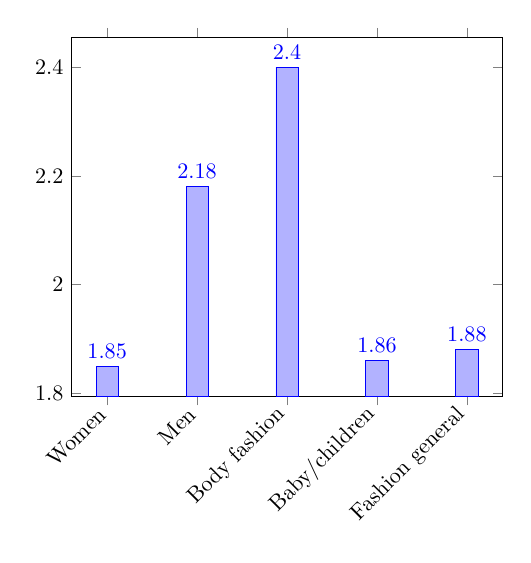
\begin{tikzpicture}[scale=0.8]
      \begin{axis}[
        ybar,
        symbolic x coords={Women, Men, Body fashion, Baby/children, Fashion general},
        x tick label style={rotate=45, anchor=east},
      ]
      \addplot +[nodes near coords] coordinates {
        (Women, 1.85)
        (Men, 2.18)
        (Body fashion, 2.40)
        (Baby/children, 1.86)
        (Fashion general, 1.88)
      };
      \end{axis}
    \end{tikzpicture}
    \caption{Conversion rate in various fashion segments}
\end{figure}

\marginpar{TODO: Conversion rate in SoBazaar?}
This figure is taken from~\cite{Jorij2012} and shows the conversion rate for
various segments in the fashion domain. The conversion rate is the portion of
users who visits a website, and reaches the target (makes a conversion) set
by the site. For most e-commerce application, SoBazaar included, a conversion
is counted when a purchase is made. The conversion rate $r$ can easily be
calulcated by $r = \frac{|Conversions|}{|Total visits|}$~\ref{nielsen2013}.
We can see that womens has the lowest conversion rate among the different
segments, indicating that there is a strong preference based shopping
tendency and that many users are \textit{browsing} and searching for the
right product. This hypthesis is strengthed by looking at the general
conversion rate in the e-commerce industry, which lies at 3\%. The potential
of a personalized recommender could in other words make browsing easier and
hence increase the conversion rate.

\begin{figure}[H]
  \begin{tabular}{cc}
    \resizebox{0.43\linewidth}{!}{
      \begin{tikzpicture}
        \pie[text=legend, rotate=60]{
          34.30/Women,
          13.43/Men,
          17.91/Generalist,
          11.94/Body,
          4.47/Shoes,
          2.98/Jeans,
          14.97/Other
        }
      \end{tikzpicture}
    }
    \resizebox{0.49\linewidth}{!}{
      \begin{tikzpicture}
        \pie[text=legend, rotate=60]{
          15/Direct,
          23/Paid,
          30/Organic,
          5/CPS,
          9/CPC,
          8/Viral or social,
          10/E-mail newsletter
        }
      \end{tikzpicture}
    }
  \end{tabular}
  \caption{Distribution of target groups and traffic sources in the fashion
  domain}
\end{figure}

Both figures are taken from~\cite{Jorij2012}, basing its results from a study
with 70 participating fashion companies with the goal of doing a complete
benchmark of the industry. In the leftmost figure we see how the different
e-commerce fashion retailers focuses their products. We observe that a large
majority of e-commerce fashion companies are targeting women - as is
SoBazaar.  Underlining the comptetative market and the need to stand out to
the customer, by e.g. having personalized recommendations.

In the rightmost figure it is shown from where the customers originate in
online retails stores. The \textit{Paid} and \textit{Organic} are synonymous
with a user entering the site via. research or ads in the search engine, and
stands for 53\% of the traffic in e-commerce fashion - highlihting the
importance of a good reputation and digital profile. Direct traffic is as low
as 15\%, compared to the e-commerce industry in general where the same number
is 22.3\% \cite{Jorij2012}. This is explained by non-fashion products often
being offered in multiple stores and the users are thus browsing multiple
sites to find the best offer. Lastly we note that the viral/social segment is
rather small at 8\%, but compared to the e-commerce industry in general at
4\%. Hence we conclude that although a small of users interacts with fashion
companies by social media, it is a more important segment in this industry
compared to e-commerce in general.

\subsection{SoBazaar, the e-commerce application}
  As briefly mentioned in the introduction chapter~\ref{sec:motivation} SoBazaar is a fashion e-commerce application for web and hand held devices.
  The application is developed by Telenor and aggregates fashion products from various brands and stores, mainly fashion related.
  Users of the application can choose to log in with their social media account on Facebook~\footnote{Facebook is an online social media service with around 1.28 billion monthly active users~\cite{facebook}} to store and share their fashion findings in the application.
  This allows the user to have one entry point to get the latest updates on fashion, and see what the user's social network is up in regards to fashion.
  When the user finds an item especially interesting and is interested in purchasing the item, the user is redirected to the store from which the product originated.

  The fact that SoBazaar utilizes Facebook and a large set of fashion stores lets the users of the application gather at one place to find users with similar taste in fashion.
  As seen from~\ref{subsec:theory} one important aspect in fashion is the feeling of belonging, which is made easy through the utilization of Facebook.

\subsection{Competitors to SoBazaar}
  \label{subsec:competitors}

	\marginpar{TODO: Extend with Asos}
	\marginpar{TODO: Extend with Kwoller}
	\marginpar{TODO: Extend with Mallzee}
	\marginpar{TODO: Mention that many new apps have popped up recently, attempting to do the same as SoBazaar}

    As seen from~\ref{subsubs:fashionInEcom} SoBazaar is not the only e-commerce application for fashion, and has therefore some competitors.
    SoBazaar is built up of a collection of e-commerce store front applications and social interactions, but SoBazaar is not the first of its kind.
    There is a set of other similar applications providing the user with similar possibilities as SoBazaar.
    This section will be used to explore some of these systems, and look into their strengths and weaknesses regarding item recommendation for the user.

\subsubsection{Myntra} % (fold)
\label{par:myntra}
    "Myntra.com is a one stop shop for all your fashion and lifestyle needs" - about Myntra~\cite{myntra}.

    Myntra is one of India's largest e-commerce stores for fashion and aims to  provide a hassle free shopping experience for the user.
    They aim to bring the newest and most in-season fashion products available to the user trough the web store front.
    The brand base of Myntra consists of 500 leading brands from both inside and outside India.

    The web page uses a set of recommendation approaches to inform the user of what they might like, and to increase the user's awareness of different kinds of items. Such as, similar item and most popular.

    \begin{figure}[H]
        \centering
        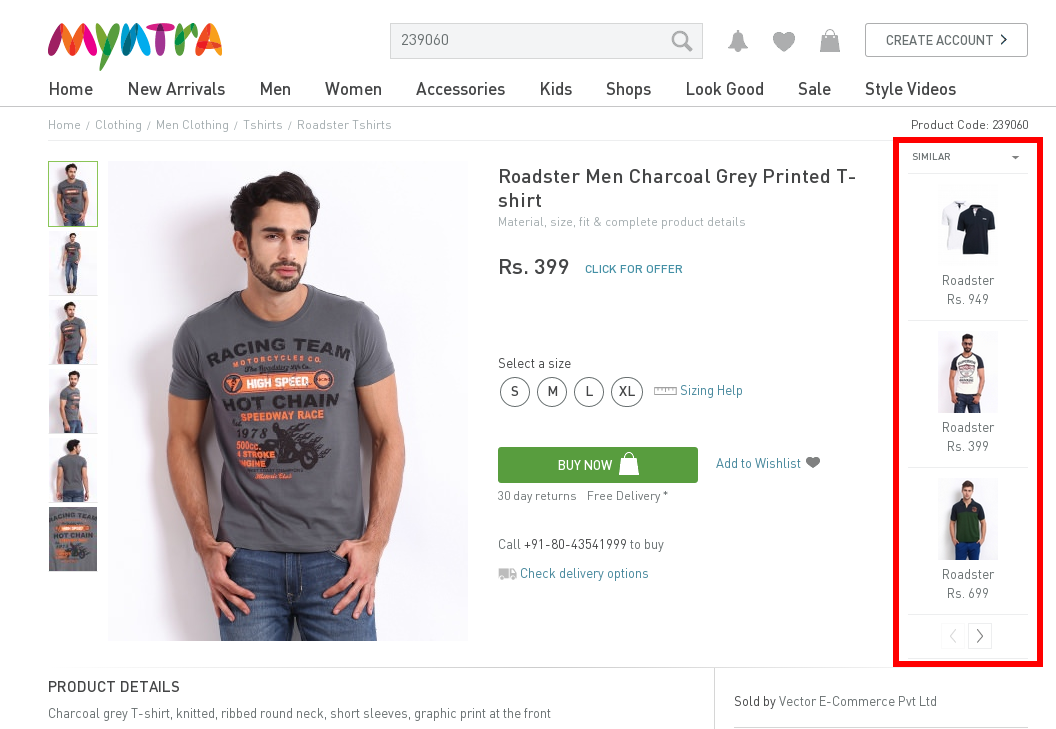
\includegraphics[width=5in]{image/myntiaSimilarExample.png}
        \caption[Example of Myntra's "similar item" approach]{In this figure we can see in red how Myntra is suggesting items which are similar to the item the user is currently looking at}
        \label{figure:myntiaSimilarEx}
    \end{figure}

    \begin{table}[H]
        \centering
        \begin{tabularx}{\linewidth}{>{\parskip1ex}X@{\kern4\tabcolsep}>{\parskip1ex}X}
            \toprule
            \hfil\bfseries Strengths
            &
            \hfil\bfseries Weaknesses
            \\\cmidrule(r{3\tabcolsep}){1-1}\cmidrule(l{-\tabcolsep}){2-2}
            %Strengths
	        Suggest similar items connected to the currently viewed \par
            Popular list for the different brands and stores \par
            Ability to add item to a "want list"\par
            &
            %Weaknesses
            No personalized recommendations \par
            \\\bottomrule
        \end{tabularx}
        \caption[Recommendation related strengths and weaknesses of Myntra~\cite{myntra}]{This table is the list of the recommendation related strengths and weaknesses of the e-commerce fashion web site Myntra~\cite{myntra}}
        \label{table:ecommerceMyntra}
    \end{table}
% paragraph myntra (end)

\subsubsection{Lyst} % (fold)
\label{par:lyst}
    "Lyst.com is a fashion shopping site that gives you your own shopping experience, so you can discover more of the fashion you love" - About Lyst~\cite{lyst}.

    Lyst offers items from thousands of the leading brands and stores of the world.

    The site allows the user to follow different stores or brands to receive the latest items they have to offer.
    The user is given a personalized "stylefeed", which displays items from the different brands or stores the user is following.
    It is also possible for the user to add items to the their profile.

    On first login the user is presented with a set of brands and store the user can like or dislike, to get the "stylefeed" started.
    On access of an item, the user is presented with related items, and the ability to add the item to a collection.
    When the user wants to buy an item, the site will redirect the user to the store selling the item.

    \begin{table}[H]
    	\centering
        \begin{tabularx}{\linewidth}{>{\parskip1ex}X@{\kern4\tabcolsep}>{\parskip1ex}X}
        \toprule
        	\hfil\bfseries Strengths
            &
            \hfil\bfseries Weaknesses
            \\\cmidrule(r{3\tabcolsep}){1-1}\cmidrule(l{-\tabcolsep}){2-2}
                    Can follow brands and stores \par
                    Connected with facebook \par
                    Ability to add item to a "want list" \par
                    "Stylfeed" based the user's follow list \par
                    Show related items \par
                    &
                    Limited personalized recommendations \par
                    \\\bottomrule
                \end{tabularx}
        \caption[Recommendation related strengths and weaknesses of Lyst~\cite{lyst}]{This table is the list of the recommendation related strengths and weaknesses of e-commerce fashion web site Lyst~\cite{lyst}}
        \label{table:ecommenreceLyst}
    \end{table}
% paragraph lyst (end)

\subsubsection{Farfetch} % (fold)
\label{par:farfetch}
    "farfetch.com forms the hub of a global fashion community that unites independent boutiques around the world with fashion lovers" - About Farfetch~\cite{Farfetch}

    Farfetch is a collection of over 1000 boutiques from all over the world gathered on one web page.
    The user can shop directly on the page, and get the item delivered to the doorstep with only one checkout process.

    When browsing an item the user is presented with a set of recommendations related to the current item, and previous browsing history.
    The item can be added to a "want list" or to the shopping chart.
    \begin{figure}[H]
        \centering
        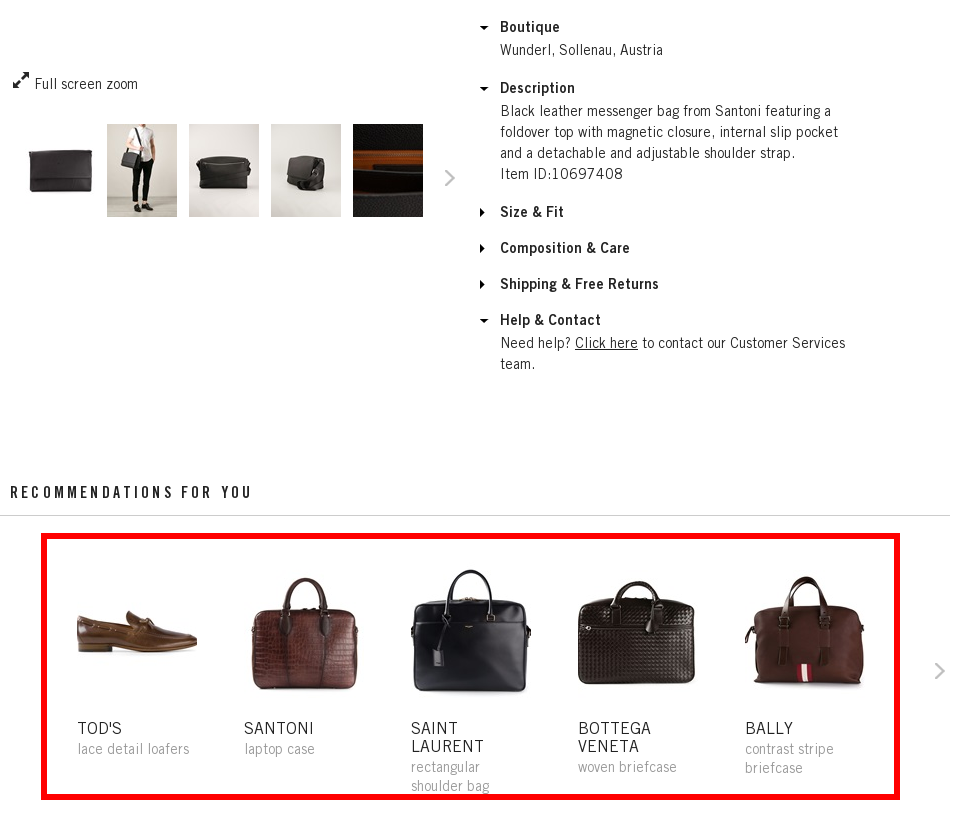
\includegraphics[width=5in]{image/farfetchedRecommendationExample.png}
        \caption[Example of Farfetch's recommendations]{In this figure we can see in red how Farfetch is recommending items which might be of interest to the user. As we can see the first item is a shoe, which was the last item accessed by the user, the next four items are related to the currently viewed item}
        \label{figure:farfetchedRecommendationExample}
    \end{figure}
    \begin{table}[H]
        \centering
        \begin{tabularx}{\linewidth}{>{\parskip1ex}X@{\kern4\tabcolsep}>{\parskip1ex}X}
        	\toprule
        	\hfil\bfseries Strengths
        	&
        	\hfil\bfseries Weaknesses
        		\\\cmidrule(r{3\tabcolsep}){1-1}\cmidrule(l{-\tabcolsep}){2-2}
        		%Strengths
                Ability to add item to a "want list" \par
                A feed with the most popular items \par
                A feed with new items \par
                A list of recommendations for the user \par
            	&
            	%Weaknesses
                No option to follow other users \par
             \\\bottomrule
        \end{tabularx}
        \caption[Recommendation related strengths and weaknesses of Farfetch~\cite{Farfetch}]{This table is the list of the recommendation related strengths and weaknesses of e-commerce fashion web site Farfetch~\cite{Farfetch}}
        \label{table:ecommenreceFarfetch}
    \end{table}
% paragraph farfetch (end)

\subsubsection{MyHabit} % (fold)
\label{par:myhabit}
    "MyHabit is a private fashion sale site offering up to 60% off hand-picked selections from designer and boutique brands." - About MyHabit~\cite{MyHabit}

    MyHabit was founded by Amazon in response to the desire from the users of Amazon to shop fashion in an easy manner.

    The site displays a feed.
    This feed is fed by a team from MyHabit, and is constantly updating with new sales and new products.
    The items put into the feed are handpicked.

    When browsing items on MyHabit, other similar items are suggested to the user.
    \begin{table}[H]
                    \centering
                    \begin{tabularx}{\linewidth}{>{\parskip1ex}X@{\kern4\tabcolsep}>{\parskip1ex}X}
                    \toprule
                    \hfil\bfseries Strengths
                    &
                    \hfil\bfseries Weaknesses
                    \\\cmidrule(r{3\tabcolsep}){1-1}\cmidrule(l{-\tabcolsep}){2-2}
                Shop on site \par
                Similar items \par
             &
                No personalized recommendations \par
            \\ \bottomrule
        \end{tabularx}
        \caption[Recommendation related strengths and weaknesses of MyHabit~\cite{MyHabit}]{This table is the list of the recommendation related strengths and weaknesses of e-commerce fashion web site MyHabit~\cite{MyHabit}}
        \label{table:ecommenreceMyHabit}
    \end{table}
% paragraph myhabit (end)

\subsubsection{Competitors Recommendation Overview} % (fold)
\label{par:competitors_recommendation_overview}
    In table~\ref{table:ecommerceCommpetiros} we see that there is a very low count of fashion related e-commerce applications, which actually produces personalized recommendations for their users.

    Most of applications are taking a simpler approach when making recommendations for the user, like most popular or similar items.
    There is no obvious relation between recommendations and that the site has a form of "want list", but the system which allows the users to follow each other are usually not in-application-purchase-applications.

    There where no indications of the "want list" being used directly to some personalized recommendations and neither was it any indication that the "follow list" of other users helped produce any personalized recommendations, other than recommending items from the followed user's feed.
    The "follow list" was also in some cases used to suggest other users to follow.
    The "want list" was primarily there so that the user could go back to a liked item, and maybe interact with it later.
    \begin{table}[H]
        \centering
        \begin{tabular}{l l l l l l l}
            \toprule
            Competitor &
            \multicolumn{1}{l}{\parbox{1.3cm}{ In App \\ Purchase}} &
            \multicolumn{1}{l}{\parbox{1.0cm}{ Most \\ Popular}} &
            \multicolumn{1}{l}{\parbox{1.0cm}{ Similar \\ Items}} &
            \multicolumn{1}{l}{\parbox{1.0cm}{ Want \\ List}} &
            \multicolumn{1}{l}{\parbox{1.9cm}{ Follow \\ Other Users}} &
            \multicolumn{1}{l}{\parbox{2.6cm}{ Personalized \\ Recommendations}} \\ \midrule

            Myntra  & \cmark & \cmark & \cmark & \cmark & \xmark & \xmark \\
            Flink   & \xmark & \cmark & ?? & \cmark & \cmark & \xmark \\
            Lyst    & \xmark & \cmark & \cmark & \cmark & \cmark & \xmark \\
            Motilo  & \xmark & \cmark & \xmark & \cmark & \cmark & \xmark \\
            Farfetch & \cmark & \cmark & \cmark & \cmark & \xmark & \xmark/\cmark~\tablefootnote{How the recommendations are produced is not mentioned} \\
            ModCloth  & \cmark & \cmark & \cmark & \cmark & \xmark & \xmark \\
            UsTrendy  & \cmark & \cmark & \cmark & \cmark & \xmark & \xmark \\
            Polyvore  & \xmark & \cmark & \cmark & \cmark & \cmark & \xmark \\
            Clothia  & \xmark & \cmark & \cmark & \cmark & \cmark & \xmark \\
            Trendabl  & \cmark & \cmark & \cmark & \cmark & \cmark & \xmark \\
            Zalando  & \cmark & \cmark & \cmark & \cmark & \xmark & \xmark \\
            Ellos  & \cmark & \cmark & \cmark & \cmark & \xmark & \xmark \\
            LookBook  & \xmark & \cmark & \cmark & \cmark & \cmark & \xmark \\
            Fahsiolista  & \xmark & \cmark & \xmark & \cmark & \cmark & \xmark \\
            ShopStyle  & \xmark & \xmark & \cmark & \cmark & \xmark & \xmark \\
            MyHabit  & \cmark & \xmark & \cmark & \xmark & \xmark & \xmark \\
            \bottomrule
        \end{tabular}
        \caption{Properties of different e-commerce application}
        \label{table:ecommerceCommpetiros}
    \end{table}
    Show in the table~\ref{table:ecommerceCommpetiros} above is the list of the different properties of some of the different competitors to SoBazaar. The properties are in regards of their recommendation ability, and how they let their user expand their item set
    A more complete list can be found in the appendix~\ref{app:sec:soCompetitors}.

% paragraph competitors_recommendation_overview (end)

% mtodo
% Diskusjon
%   behold 3 resten til appendix
      % utdyp om SoBazaar, hvordan passer de inn
      % Bruk data til å beskrive at det vi driver med er viktig.
%   Hvborfor har vi dette?
%   Dert er få anbefalinger
%   Dollars er et lukurativt market

  % Heri satte utropstegn ved:
  %   Flink
  %   Lyst og
  %   Motilo

\subsection{Fashion Recommender Systems}
    This subsection will look at different methods other fashion related systems have used to recommend fashion related products to the user.

\subsubsection{Photograph based approach}
    Fashion and the products it regards are highly dependent on visuals.  A fashion
    product would not be very interesting if no one saw it.  An approach to use the
    importance of how the product looks regarding recommending is to utilize images
    of the product.  Fashion Coordinates Recommender System Using Photographs from
    Fashion Magazines~\cite{Iwata:2011} is a system doing this.  They teach their
    system by using fashion magazines with full body images.  They segment the
    image into two parts, top and bottom.  From this the system learns which top
    matches to which bottom and collects visual features of the products.  From
    this the system can recommend other tops to go with a selected bottom, or other
    way around.  The proposed system scored better\footnote{Accuracy of 50\% on the
    top 5 suggested items, whereas naive and random managed 18\% and under 5\%
    respectively} than both a more naive approach and a random selection.  Runtime
    was at 0.04 seconds per recommendation.

\subsubsection{Hot-or-not}
    A recommender system called SuitUp~\cite{SuitUp} did a survey on some of their potential users.
    One interesting finding was that many of the users enjoyed the Hot-or-Not feature of the system.
    This feature gives the user a set of items and the option to either like or dislike.
    This did not only make the participants in the survey more engaged in the system, but also produced ratings, both negative and positive, for the system.
    For cold-start users and in a cold-start system this extra information and ratings make it much easier to make recommendations for the users.

\subsubsection{Scenario-Oriented Recommendation}
    Shen et al.~\cite{Shen:2007:AIG:1216295.1216368} proposed a recommender system which produce recommendations not only based on the metadata of the products, but also on user written input.
    Knowledge used to handle the user input, is derived from Open Mind Common Sense~\cite{Singh02openmind}.

    The user uploads his or her clothes and adds brand (e.g.Nike), type (e.g.jeans), material and a description about the item (e.g."I put these on when I get home").
    The systems makes recommendations based on the scenario the user is needing help to find suiting clothes to wear.
    The typical use case of the system is when a user is unsure about what to wear under different circumstances, but knows something about the scenario or occasion the clothes will be worn in.
    For instance: "I am going to the beach".
    It is also possible to interact with other users and the system relates similar users.

    The different describing fields about the items are given a six-tuple style value.
    The six tuples are: luxurious, formal, funky, elegant, trendy and sporty, where each is given a value from 0 to 10 based on how much the describing field of the items is the current tuple.
    The different describing fields are given a default value, which can be changed by the user if that this necessary. But it seems like this has to be done for all brands, material and type manually to initialize the system.

    This is an interesting approach to fashion and clothes recommendations but the need for user scenario input and a six-tuple description of the different describing fields, might not be desirable for the user or the system administrator in the long run.

    Yu-Chu et al.~\cite{Yu-Chu:2012:PCS:2376365.2376961} and Ying et al.~\cite{Ying2011} are other similar systems. Ying et al.~\cite{Ying2011} made a recommender based on the a similar concept, namely, what to wear in different situations.
    The system recommends two sets of top-to-toe clothing based on the current season, the occasion and the items the user has uploaded.
    The uploaded items must be given a set of descriptions, including the occasion to use the item.

    To recommend, the system uses the user profile of the user, which describes the interests of the user and the information given by the user about the different items in his or hers wardrobe.

\subsubsection{Photograph Recommendation Integrated with Occasion} % (fold)
\label{par:photograph_recommendation_integrated_with_occasion}
    Liu et al.~\cite{Liu:2012:HMC:2393347.2393433} combined the two approaches from Iwata et al.~\cite{Iwata:2011} and Ying et al.~\cite{Ying2011} and Shen et al.~\cite{Shen:2007:AIG:1216295.1216368} and suggested a system which recommend clothes both based on the photographies and the occasion the clothes are to be worn.

    They do this by incorporating fashion rules like, what can you wear to which occasion, and what can you wear as a complete set to different occasions.
    The recommender learn the clothing recommendations through a latent support vector machine framework.
    They use this framework to match four potential functions: visual features vs. attribute, visual features vs. occasion, attributes vs. occasion and attribute vs. attribute.
    These are used together in a scoring function for clothing recommendation.

    Their system preformed better than the baselines, but was highly dependent on the human detection accuracy, since the learner was learning from fashion photographs.
% paragraph photograph_recommendation_integrated_with_occasion (end)
